\subsection{有効粘度の評価}
Fig.\ref{fig:estimate_eff_viscocity}はせん断速度と有効粘度の関係を表す.

    \begin{figure}[H]
        \centering
        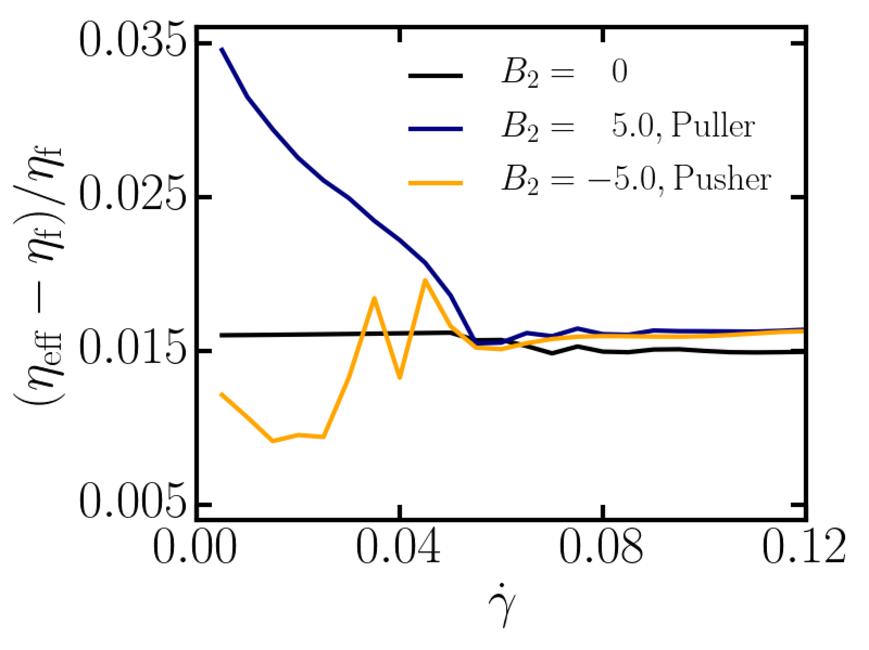
\includegraphics[scale=0.5]{/Users/taiga/Projects/lab/thesis/components/chapter4/figs/gammadot_vs_eff_viscosity.pdf}
        \caption{せん断速度と有効粘度の関係}
        \label{fig:estimate_eff_viscocity}
    \end{figure}

\noindent
このグラフから,せん断速度が小さい領域では,$B_2 > 0$のPuller型は有効粘度を大きくする方向に,
$B_2 < 0$のPusehr型は有効粘度を小さくする方向にはたらいていることが分かる.
また,せん断速度が大きい領域ではsquirmerの種類によらず,ほぼ等しい有効粘度を示していることが分かる.
Rafa\"iらによるPuller型のsquirmerであるクラミドモナスを用いたせん断速度と有効粘度の関係を検証する実験結果によると,
せん断速度が小さい領域では系の有効粘度を大きくする方向にはたらき,
せん断速度が大きい領域では,せん断速度に関わらずほぼ等しい有効粘度を示すことが分かっている\cite{effective_viscosity}.
また,MartinezaらによるPusher型のsquirmerであるE. Coli.を用いたせん断速度と有効粘度の関係を検証する実験結果によると,
同様に,せん断速度が小さい領域では系の有効粘度を小さくする方向にはたらき,
せん断速度が大きい領域では,せん断速度に関わらずほぼ等しい有効粘度を示すことが分かっている\cite{e_coli_experiment}.
これらの実験結果と今回のシミュレーション結果は定性的に一致していると言うことができる.

    \begin{figure}[htbp]
        \centering
        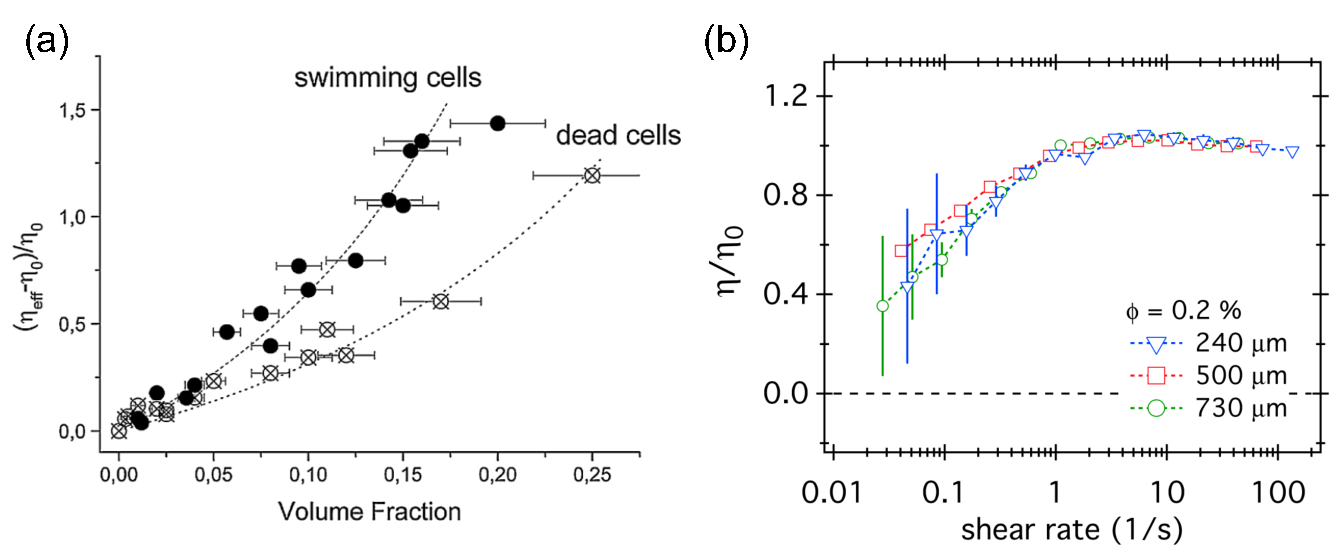
\includegraphics[scale=0.7]{/Users/taiga/Projects/lab/thesis/components/chapter4/figs/previous_effective_viscosity.pdf}
        \caption{(a)クラミドモナスのせん断速度と有効粘度の関係,(b)E. Coli.のせん断速度と有効粘度の関係}
    \end{figure}
